\section{Publish/Subscribe-Systeme}
\label{chap:grundlagen:pubsub}
Publish/Subscribe-Systeme sind Forschungszweck vieler wissenschaftlicher Arbeiten \cite{Liu2003Survey, Banerjee2001Comparative}. Themen wie Sicherheit \cite{FiegeSecurity}, ``Quality of Service'' \cite{BeFiMu2006PubSubQoS} oder Verteilungsoptimierung \cite{Muhl2002LargeScale, Castro2002Scribe} sind gut erforscht und beschrieben.

Publish/Subscribe-Systeme lassen sich konzeptionell als Event-Systeme betrachten. Auf Grund ihres Aufbaus und der Skalierung  in orthogonalen Dimensionen\index{Publish/Subscribe!orthogonale Dimensionen} \emph{Raum}, \emph{Zeit} sowie \emph{Verarbeitungsmodell} eignen sich diese gut zur Verteilung von Events in dezentralen Umgebungen \cite{PatrickTh2003Many}. Diese Dimensionen werden im Folgenden genauer erläutert.

\begin{figure}[htbp]
\centering
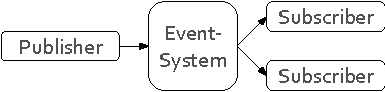
\includegraphics{grafics/pubsub_black_box.pdf}
\caption{Schema eines Publish/Subscribe-Systemes.}
\label{fig:pubsub_black_box}
\end{figure}

\paragraph{räumliche Trennung}
Das Event-System trennt Publisher und Subscriber voneinander, wie es in Wie in \Fref{fig:pubsub_black_box} dargestellt. Diese Trennung bezieht sich nicht nur auf verschiedene Komponenten einer Applikation, sondern kann auch über Applikationsgrenzen oder gar Rechnergrenzen gehen.

Diese Trennung kann so weit gehen, dass verschiedene Publish/Subscribe-Systeme miteinander kommunizieren können. Pietzuch gibt einen Vorschlag für eine generische API\index{Publish/Subscribe!generische API} für Publish/Subscribe-Systeme und unterteilt die Kompabilität verschiedener Systeme in drei Level. Das höchste Level beschreibt einen Datenaustausch der an XML-RPC angelegt ist \cite{PiEyKoSh2007-PubSubAPI}.

\paragraph{zeitliche Trennung}
Publisher und Subscriber sind in ihren Aktionen mit dem Event-System zeitlich getrennt. Ein Publisher muss kein Wissen über Subscriber haben und umgekehrt. Dies bedeutet dass sich ein Subscriber am System anmelden kann obwohl kein Publisher vorhanden ist. Für Publisher gilt dies analog. Bei einem Fernaufrufsystem wie \emph{message-passing} ist dies nicht möglich, da die Gegenseite bekannt sein muss.

\paragraph{asynchrone Verarbeitung}
Das Senden einer Nachricht ist für den Publisher nicht blockierend und entspricht dem Kommunikationsparadigma ``send and forget''. Subscriber warten zudem nicht aktiv auf neue Nachrichten, sondern werden per Callback über neue Nachrichten informiert. Damit wird die Verarbeitung vom Event-System aus getriggert.


\subsection{Arten von Publish/Subscribe-Systemen}
Publish/Subscribe-Systeme sind grundsätzlich in die zwei Varianten  \emph{kanalisiert} und \emph{filterbasiert} einzuteilen. Deren unterschiedliche Arbeitsweise wird in diesem Kapitel erklärt.

\subsubsection{Kanalbasiert}
\label{chap:grundlagen:pubsub:kanalbasiert}
Nachrichten in kanalbasierten\index{Publish/Subscribe!kanalbasiert} Systemen werden im Kontext von Kanälen oder Themen behandelt. Nachrichten können nur in Verbindung mit einem Thema an das System übergeben werden. Clients können sich für verschiedene Kanäle einschreiben und erhalten nur diese Nachrichten.

Kanalbasierte Systeme können sehr gut optimiert werden, da die Anzahl der Kanäle und deren Art zur Erstellungszeit meist bekannt ist. Selbst wenn zur Laufzeit neue Kanäle hinzugefügt werden, geschieht dies ebenfalls strukturiert und dient der internen Optimierung des Systems. Durch die Gruppierung der Nachrichten müssen insgesamt weniger Nachrichten verschickt werden.

Filterungen sind in diesem Systemen meist nur clientseitig effizient möglich. Clients können die empfangenen Nachrichten filtern und unpassende Nachrichten verwerfen. Wird eine Filterung durch strukturierte Kanalnamen ermöglicht, kann die Anzahl der zu versendenden Nachrichten reduziert werden.

Um das System im Voraus filtern zu lassen, müsste ein geeigneter Filter bei der Anmeldung übergeben werden. Damit das Event-System die Nachrichten filtern kann, müssen diese in einem vom System lesbaren Format vorliegen. Dies bedeutet, dass das Event-System und die Clients stärker gekoppelt sind oder dass durch selbst beschreibende Nachrichtenformate die Nachrichtengröße aufgebläht wird.\\
Pietzuch zeigt mit einem System aus XML basierten Nachrichten und XPath Filter eine interessante Variante die Filterung bereits im Publish/Subscribe-System zu ermöglichen \cite{PiEyKoSh2007-PubSubAPI}.

Können keine selbst beschreibende Nachrichtenformate genutzt werden, so müssen dem Event-System Callbacks zur Filterung zur Verfügung stehen. Diese Callbacks können jedoch erst auf Clientseite ausgeführt werden, was einen Transport der Nachricht zum Client bedingt. Dies widerspricht jedoch der Idee der Nachrichtenvermeidung durch Filterung.

Ein prominenter Vertreter dieser Art ist Scribe \cite{Castro2002Scribe}, dessen Funktionsweise in \Fref{chap:related:scribe} genau beschrieben wird.

\subsubsection{Filterbasiert}
\label{chap:grundlagen:pubsub:filterbased}
In filterbasierten\index{Publish/Subscribe!filterbasiert} Systemen gibt es streng genommen nur einen einzigen Kanal. Eine Nachricht besteht aus meheren Attributen mit verschiedenen Wertebereichen. Die Anmeldung erfordert die Übergabe eines Prädikates, welches die Attribute und Wertebereiche eingrenzt. Das Event-System stellt dem Client nur anhand diesem Prädikat gefilterte Nachrichten zu. In solchen Systemen ist es obligatorisch, dass das System die Nachrichtenstruktur kennen muss, beziehungsweise müssen diese mit filterbaren Metadaten angereichert werden \cite{PiEyKoSh2007-PubSubAPI}.

Filterbasierte Systeme sind nicht im gleichen Ausmaße optimierbar wie kanalbasierte Systeme, da jeder Client potentiell alle Nachrichten empfangen kann. Durch eine Anpassung der Filter sind diese Systeme jedoch flexibler in der Benutzung. Die Definitionen der Attribute und deren Wertebereich haben eine Auswirkung auf den Systemaufbau. Sind diese zur Laufzeit änderbar, so muss das System weitaus generischer arbeiten als dies bei einer feststehenden Menge an Attributen.

\subsection{Umsetzung verteilter Publish/Subscribe-Systeme}
Anhand Scribe (kanalbasiert) \cite{Castro2002Scribe} und Mercury (filterbasiert) \cite{Bharambe2004Mercury} wird die Umsetzung der in diesem Kapitel vorgestellten Arten in strukturierten Overlay-Netzwerken beschrieben. Obwohl sich \ac{m2etis} im jetzigen Entwicklungsstand auf kanalbasierte Systeme beschränkt \cite{Fischer2010a}, kann der Algorithmus hinter Mercury interessante Einblicke und Ideen liefern.

Da ausgefallene Knoten in solchen Netzwerken nicht aktiv erkannt werden, müssen Anmeldungen periodisch erneuert werden. Dies stellt sicher, dass die Nachrichten vom Netzwerk automatisch über andere Knoten geleitet werden und sich so der logische Multicast-Tree wieder aufbauen kann. Dennoch können in der Zwischenzeit Nachrichten verloren gehen.

\subsubsection*{Kanalbasiert am Beispiel von Scribe}
\label{chap:related:scribe}
Eine Umsetzung von Publish/Subscribe-Systemen in verteilen Systemen, ist der Aufbau eines Multicast-Trees\index{Multicast-Tree}, d.h. eines durch die Knoten im Netz gebildeten Baumes in dem die Nachrichten verteilt werden. Hierbei wird pro Kanal ein eigener Multicast-Tree aufgebaut. Am Algorithmus von Scribe wird diese Struktur beschrieben.

Scribe basiert auf dem strukturierten Overlay-Netzwerk Pastry \cite{Rowstron2001} und erzeugt einen vom Subscriber zum Publischer aufgebauten Baum \emph{reverse path forwarding tree} \cite{Dalal1978}.

\begin{figure}[htbp]
\centering
\resizebox{\textwidth}{!}{%
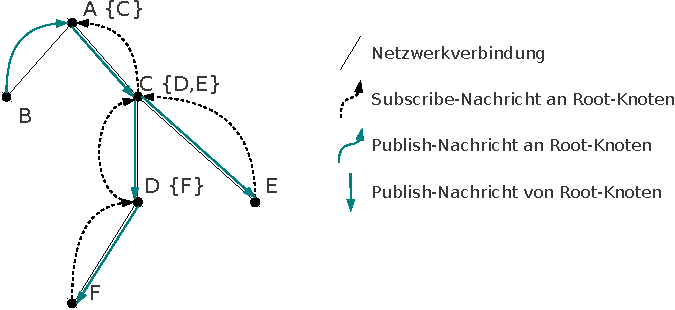
\includegraphics{grafics/multicast_tree.pdf}}
\caption{Schema eines Multicast-Trees}
\label{fig:multicast_tree}
\end{figure}

\Fref{fig:multicast_tree} zeigt ein Netzwerk mit den sechs Knoten A-F. Die Verbindungen der Knoten werden durch dünne schwarze Linien dargestellt. Beispielsweise hat Knoten C Verbindungen zu A, B, D und F.\\
Der Multicast-Tree benötigt einen Knoten, der die Wurzel (im Folgenden \emph{Root-Knoten} genannt) darstellt. Aus Hashwert des Kanalnamens wird ein Schlüssel berechnet. Derjenige Knoten, der aufgrund der Netzwerkmetrik für diesen Schlüssel zuständig ist, wird Root-Knoten des Kanals. Im abgebildeten Falle ist dies Knoten A.\\
Weiterhin hält jeder Knoten eine Liste bei ihm angemeldeter Knoten. In der Abbildung wird diese Liste durch geschweifte Klammern nach der Knotenbezeichnung dargestellt.

\paragraph*{Anmelden}
Knoten F sendet eine \emph{subscribe}-Nachricht an A. Diese Nachrichten sind in der Grafik durch gebogene gestrichelte schwarze Verbindungslinien mit Pfeil dargestellt. Das Netzwerk würde diese Nachricht über Knoten D und C an A routen. Knoten D lässt die Nachricht terminieren und trägt F in die Liste der Subscriber ein. Knoten D sendet nun selbst eine subscribe-Nachricht an A. C, über den die Nachricht geroutet wird, terminiert diese, trägt D in die Liste ein und sendet selbst eine subscribe-Nachricht an A. A erhält nun diese Nachricht und trägt C in die Liste ein. Damit sind nun insgesamt drei Nachrichten verschickt worden.\\
Wenn sich Knoten E für den Kanal einschreibt, wird die subscribe-Nachricht an A über den Knoten C geleitet. Dieser terminiert die Nachricht und fügt E der Liste hinzu. Da C selbst angemeldet ist, muss keine weitere Nachricht versendet werden.

Scribe fordert periodische Anmeldungen zur Erhöhung der Fehlertoleranz. Ist ein Knoten ausgefallen, routet das Netzwerk die Nachrichten über andere Knoten. Damit kann der Multicast-Tree wieder aufgebaut werden.

\paragraph*{Abmelden}
Der Austritt aus einem Kanal erfolgt ähnlich zur Anmeldung. Die Nachricht läuft nur bis zum nächsten Knoten und terminiert dort. Der Knoten entfernt den Sender der Nachricht aus seiner Liste und sendet selbst nur eine \emph{unsubscribe}-Nachricht, wenn die Liste leer ist und er selbst nicht angemeldet ist.

\paragraph*{Publizieren}
In \Fref{fig:multicast_tree} möchte Knoten B eine Nachricht im Kanal publizieren. B sendet darauf eine Nachricht an den Root-Knoten A, da dieser für diesen Kanal zuständig ist (gebogene türkise Linie). Nun sendet A diese Nachricht an alle Knoten in seiner Liste (gerader türkise Linie mit Pfeil). Dies ist in der Abbildung nur Knoten C. Dieser sendet sie weiter an D und E. E gibt diese Nachricht direkt an die Applikation weiter, während D die Nachricht an F schicken muss.


\paragraph*{Schwächen}
Hierbei ist klar ersichtlich, dass zusätzliche Nachrichten verteilt werden müssen, wenn Knoten F eine Nachricht im Kanal publizieren möchte. Diese Nachricht muss erst von Knoten F zu Knoten A wandern, damit A diese Nachricht wieder über die anderen Knoten zurücksendet. Optimierte Versionen dieses Algorithmus können hier ansetzen und zu publizierende Nachrichten nicht mehr an den Knoten senden, der ihnen diese Nachricht geschickt hat. So würde C die Nachricht nur noch an E weiterleiten.

\paragraph*{Filterung}
Eine Filterung der Nachrichten ist möglich. Im einfachsten Falle wird das Prädikat der Anmeldung bei jedem angemeldeten Knoten geprüft. Werden die Prädikate mit der Anmeldungsinformation verbunden, können diese an den Zwischenknoten zu einem generellem Prädikat kombiniert werden.

\paragraph*{Ähnliche Algorithmen}
Bayeux \cite{Zhuang2001} ist ein ähnliches System, jedoch auf Basis des Overlay-Netzwerkes Tapestry \cite{Zhao2004Tapestry}. Tapestry entspricht auch der generischen API, somit stellt dies keinen Unterschied zu Pastry dar. Im Gegensatz zu Scribe, wird bei Bayeux der Multicast-Tree vom Root-Knoten aus aufgebaut. Aufgrund der unterliegenden Routingstruktur des genutzten Overlay-Netzwerkes können sich diese Pfade unterscheiden.\\
\ac{von} geht hier einen ähnlichen aber vom Aufbau des Netzwerkes anderen Ansatz. In diesem Netzwerk ist ein Nachbar in der virtuellen Welt direkt auch ein Nachbar im Netzwerk. Der Nachrichtenaustausch erfolgt nur mit den Nachbarn \cite{Hu2006VON}. \ac{vast} \cite{Backhaus2007Voronoibased} greift das Konzept von \ac{von} auf und testet eine Implementierung auf OpenSIM \cite{Baumgart2007OverSim}.



\subsubsection{Filterbasiert am Beispiel von Mercury}
\label{chap:related:mercury}
Zur besseren Vorstellung einer Umsetzung für filterbasierte Publish/Subscribe-Systeme\index{Publish/Subscribe!filterbasiert} wird im folgenden Kapitel Mercury \cite{Bharambe2004Mercury} vorgestellt. Obwohl \ac{m2etis} ein kanalbasiertes Publish/Subscribe-System darstellt \cite{Fischer2010a}, ist es sinnvoll eine möglich Umsetzung eines filterbasierten Systems zu beschreiben um die grundlegenden Unterschiede der Systeme genauer auszuarbeiten. 

\paragraph*{Arbeitsweise}
Im System gibt es eine Menge an Attributen, die ihrerseits einen definierten Wertebereich haben. Jedes Attribut wird durch einen eigenen Verbund aus Knoten, den sogenannten \emph{Hub}, bearbeitet. Der Wertebereich ist dabei nicht zwingend symmetrisch auf die Knoten verteilt.

\paragraph*{Anmelden}
Eine Subscription $S$ ist ein Tupel aus Filterbedingungen über die Attribute (z.B. $S := (5 < x <= 20; y = 15)$) sowie Kontaktinformationen des Knotens. $S$ wird an einen beliebigen Knoten eines Hubs gesendet, der für das Attribut aus der Filterbedingung mit der größten Selektivität zuständig ist. Im Beispiel ist dies Attribut $y$. Im Hub wird $S$ nun zu dem Knoten weitergereicht, der den Wertebereich der Filterung abdeckt. Dort wird $S$ in einer Liste gespeichert.

\paragraph*{Publizieren}
Eine Publikation $P$ ist ebenfalls ein Tupel mit bestimmten Werten der Attribute (z.B. $P := (x = 10; y = 0)$). $P$ wird an \emph{alle} Hubs gesendet und dort zum zuständigen Knoten weitergereicht. Dieser prüft nun die Liste der gespeicherten Subscriptions gegen die neue Publikation. Stimmen beide überein, so wird $P$ an den eingeschriebenen Knoten weitergeleitet.

%\paragraph*{Offene Punkte}
%\begin{itemize*}
%\item Änderung der Attribute zur Laufzeit?
%\item Auswahl der Knoten für einen Hub?
%\item Aufteilung der Wertemenge auf die Knoten?
%\end{itemize*}

\paragraph*{Ähnliche Algorithmen}
Mirinae ist ebenfalls ein filterbasiertes Publish/Subscribe-System, stellt den Wertebereich eines Attributes jedoch als Hyperwürfel dar. Eine automatische Anpassung dieser Aufteilung ermöglicht eine schnelle Anpassung der Routingtabelle und damit einen kurzen Weg für die Nachrichten \cite{Choi2005Mirinae}.
